\section{Reflektion}
\begin{frame}
	\frametitle{Refleksion}
	%Bad choices due to inexperience
	%and disagrements of subjective value of the langauge, such as readablity, resulting in half solutions
	%Should instead focus on the target groups preferences as it is their opinions is the ones that ultimately counts
	Reasons for bad decisition:
	\begin{enumerate}
    \item Manglende erfaring med emnet
    \item Uenighed omkring subjektive enmer
  \end{enumerate}
\end{frame}

\section{Creative realisation}
\begin{frame}
	\frametitle{A creative realisation}
	%Actors instead of functions, spread the responsiblity, an interesting side-effect
	%This encourages the user to model problem with actors, providing transparency of the actual working of the compiler( but not consise, as expressing as a function)
	Actors som erstatninger til funktioner
	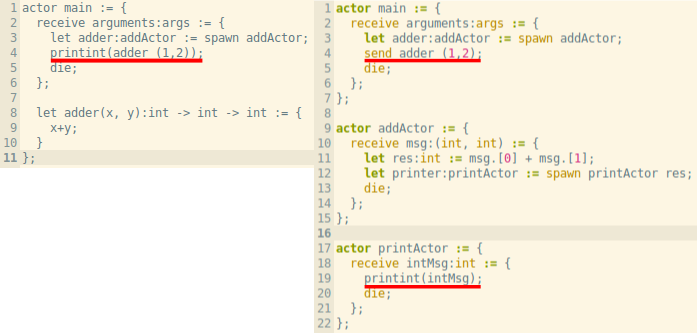
\includegraphics[width=200px]{Images/actorFunc.png}
	Men mindre koncist
\end{frame}

\section{Konklusion}
\begin{frame}
	\frametitle{Konklusion}
	%Problemformulering, actors as an solution
	Actors som en løsning
	Opfordre til at modellere problemmet med brug af actors.
\end{frame}

\section{Fremtidigt arbejde}
\begin{frame}
	\frametitle{Fremtidigt arbejde}
	Ideer and konstruktioner ikke inkluderet, endnu: 
  \begin{enumerate}
    \item Nedarving(OOP)
    \item Ny konstruktion "reply", programmøren behøver explicit at definere afsender lokalt.
    \item Envoriments og IterationSteps
  \end{enumerate}
\end{frame}

\subsection{Environments}
\begin{frame}
	\frametitle{Environments}
	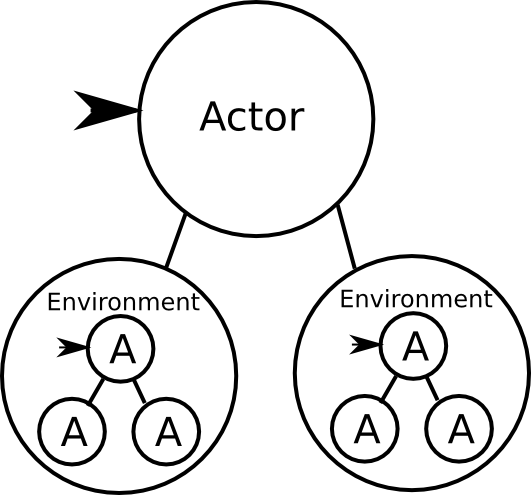
\includegraphics[width=200px]{Images/environment.png}
\end{frame}
\subsection{IterationSteps}
\begin{frame}
  \frametitle{IterationSteps}
  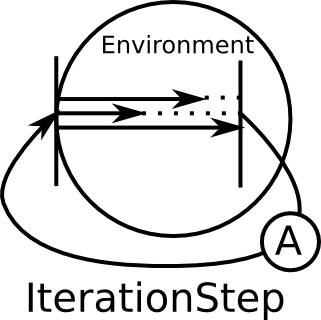
\includegraphics[width=200px]{Images/iteration.png}
\end{frame}
